The~presence of dust in space was hypothesized long ago by \citet{cassini1685} as an explanation for the~faint light on the~night sky near the~plane of ecliptic, the~zodiacal light. Dust was also observed locally, that is \textit{in-situ}, by its interaction with spacecraft since the~dawn of the~space age, when the~concern about the~risk it posed to the~spacecraft was present \citep{whipple1958meteoritic}. This chapter provides an introduction into dust detection methods in general, and into antenna detected impact ionization in particular, since it is vital for the~rest of the~present work.

\section{Remote observations}

Since dust grains in space absorb light, they are observed by extinction of light, \citep{desert1990interstellar} allowing for transmission spectroscopy, which is useful on the~galactic scale \citep{mann2010interstellar}. In terms of the~solar system, refraction, reflection, and thermal emission by dust is important, since it shows the~spatial distribution and size distribution of dust in the~zodiacal cloud \citep{allen1946spectrum,hulst1947zodiacal,leinert1981zodiacal,stenborg2018characterization,stenborg2021psp}. Measurements of luminance in principle integrate the~luminosity on a~line of sight ({LOS}) between the~observer and infinity. Most of the~luminosity originates near the~Sun, where both the~dust density and the~sunlight are the~strongest. However, as the~existence of Gegenschein shows \citep{roosen1971gegenschein}, scattering is very angle dependent. It favors smaller angles and, therefore, the~sources closer to the~observer, and makes the~inversion of LOS luminance into dust density more model dependent and ambiguous \citep{mann2004dust,kneissel1991spatial}. Observations from $\SI{1}{AU}$ are therefore limited, especially a~few angular degrees from the~Sun. The~best results are achieved with measurements closer to the~Sun, such as those of the~two Helios spacecraft \citep{leinert1981zodiacal}, which, as we mentioned previously (Eq.~\ref{eq:dust_number_density}), found the~number density of bound dust between $\SI{0.3}{AU}$ and $\SI{1}{AU}$ scaling as $n(R) \propto R^{-1.3}$. More recently, measurements of the~Wide-field Imager for Solar Probe ({WISPR}) confirmed this trend \citep{stenborg2021psp}, and even observed a~dust depletion zone within $19 \, R_{Sun} \approx \SI{0.09}{AU}$ \citep{stenborg2022psp}. The~measurements are difficult to interpret because the~luminance of dust-caused F-corona and dust-independent K-corona are hard to distinguish. 

WISPR observed many phenomena, one of them being the~clouds of spacecraft debris liberated by impacts of hypervelocity dust on the~insulating carbon foam \citep{malaspina2022clouds}. The~carbon thermal insulation is fragile, and the~debris moves slowly enough that the~light they scatter is captured in individual shots, allowing for the~estimation of their speed, which was found to be about of $1 \, \si{m/s}$. Trajectories of the~debris were also found to be curved around biased electrical antennas, which is a~motion similar to the~motion of electrons in \citeauthor{pantellini2012nano} process \citep{pantellini2012nano}, which we hypothesize might be responsible for the~double-peak signals reported on SolO in Paper~III. 


\section{Impact ionization}

\subsection{Charge generation process}

A~very fast impact of a~dust grain onto a~solid target, such as spacecraft body, releases free charges. This is because of the~great energy density at the~impact site \citep{shen2021cosmic}. At moderate relative speeds of $v \lesssim \SI{10}{kms^{-1}}$, the~ionization is mostly due to surface effects on the~grain and on the~target \citep{kissel1987ion}. At much higher speeds $v \gtrsim \SI{20}{kms^{-1}}$, the~grain is destroyed completely, and the~ionization is due to the~effects in the~bulk of the~target \citep{hornung1994shock}. For this, shock wave formation in the~target at supersonic speed is important \citep{drapatz1974theory}, which concentrates the~available energy into the~shock front, which makes up a~small volume of the~target, resulting in high volumetric energy density. 

The~first reported observation \citep{friichtenicht1964} of impact ionization followed shortly after the~development of the~first $\si{MV}$ dust accelerator \citep{friichtenicht1962}. The~charge leaving the~impact site after the~impact of carbon and iron dust grains was measured with a~preamplifier connected to a~metallic target. The~charge was observed to be quasi neutral, and the~amount of generated charge $q$ was found consistent with the~relation
\begin{equation}
    q \propto m v^3,
\end{equation}
for the~velocities  $\SI{2}{kms^{-1}} < v < \SI{15}{kms^{-1}}$, where $m$ is the~mass of the~grain and $v$ is the~impact speed. Later measurements \citep{auer1968,mcbride1999meteoroid,grun1984impact,collette2014micrometeoroid,shen2021cosmic} worked with a~more general empirical equation of 
\begin{equation}
    q \propto m^\alpha v^\gamma, \label{eq:charge_generation}
\end{equation}
and mostly found $\alpha \approx 1$ and $3 < \gamma < 5$, depending on the~speed interval and the~combination of the~grain material and the~target material. 

We note that the~amount of generated charge is random, even if $m,v,\alpha,\gamma$ are known, and Eq.~\ref{eq:charge_generation} is the~model for the~average amount of the~generated charge. The~difference between this average and the~individual data points is often significant, with a~spread of a~factor of two or more \citep{collette2014micrometeoroid,shen2021cosmic}. Due to the~randomness involved, and due to the~steep dependence on the~impact speed $v$, little information about mass $m$ is usually recovered from the~measurement of charge $q$, unless the~measurement happened in a~well controlled environment of a~laboratory.

\subsection{Laboratory simulation}

The~most successful dust accelerators are based on electrostatic acceleration principle, not dissimilar to the~ion gun. The~latest such device offers the~acceleration voltage of up to $\SI{3}{MV}$ \citep{shu20123}, allowing for speeds up to $v\gtrsim \SI{50}{kms^{-1}}$ for $r\lesssim\SI{1}{\mu m}$ grains, measuring both the~mass and the~charge state of the~grain right before it hits the~target. It not only allows for study of the~impact ionization process \citep{collette2014micrometeoroid,nouzak2018laboratory,kovcivsvcak2020effective,nouzak2021detection,shen2021electrostatic,shen2021laboratory,shen2023variability}, but also for the~study of atmospheric ablation \citep{thomas2017experimental,deluca2018ionization,deluca2022differential,tarnecki2023experimentally}. Many aspects of each impact can be measured at the~same time, as there is no limitation on the~payload nor on the~transmission capacity, such as in the~case of spacecraft experiments. Although versatile, accelerator measurements bear disadvantages: the~experiment happens in a~confined chamber in finite vacuum, the~accelerated dust grain is selected randomly from a~reservoir, and there is an intrinsic correlation between the~speed and the~mass of a~grain, given the~charge and the~accelerating voltage are constant \citep{shelton1960electrostatic}. As far as the~replication of space environment goes, the~plasma conditions (solar wind, UV illumination) can be partially replicated in laboratory \citep{shu20123,horanyi2008surface}, but the~noise level in laboratory is never achieved as low as in space. 

\subsection{Dedicated ionization detectors}

The~mechanism of impact ionization is used to detect dust impacts on spacecraft. In principle, a~surface is in a~chamber, where the~entry of charged particles is blocked by a~filter, which is however not capable of blocking the~entry of dust grains. The~surface is therefore exposed to potential dust impacts, which are the~only thinkable source of charge in the~chamber. Charge is monitored with a~bias collector in the~chamber, and whenever it appears, it is due to a~dust impact. The~first such detector was used on the~Orbiting Geophysical Observatory ({OGO}) 3 mission \citep{alexander1968zodiacal}, and was used many times in forms of variable complexity, some of them resolving the~charge and directionality \citep{grun1992galileo,grun1992ulysses,berg1969pioneer} of the~incident grains, or even allowing for spectroscopy of the~impact plasma \citep{srama2004cassini,sommer2023measuring}. Impact ionization detectors are sensitive and versatile, and they are used not only in orbit, but also on sounding rockets \citep{gunnarsdottir2019charging,trollvik2019observation} to study smoke particles in the~mesosphere. 

\subsection{Non-ionization dust detectors}

\subsubsection{Mechanical methods} 

A~penetration method was employed on Pioneer 10 and 11 \citep{humes1980results}. A~$\SI{25}{\mu m}$ and a~$\SI{50}{\mu m}$ pressurized steel cells were mounted on Pioneer 10 and 11 respectively, $234$ cells on each, counting the~impacts of dust grains fast and big enough to penetrate them, which showed by the~pressure loss in the~cell. Together, these detectors counted $182$ dust impacts, showing clearly higher abundance of dust near Jupiter and Saturn, and concluding that the~$\approx \SI{10}{\mu m}$ grains observed between the~asteroid belt and Jupiter were not circular and in the~ecliptic plane, but rather eccentric or inclined. 

An integration experiment was conducted on the~Long Duration Exposure Facility ({LDEF}) satellite \citep{love1993direct}, which consisted of a~study of $\SI{5.6}{m^2}$ aluminium plate exposed to the~near-Earth environment for nearly six years. In total $761$ craters were found on a~microscope scan, allowing for the~estimate of the~total meteoric mass accretion rate by the~Earth to $40 \pm 20 \, \si{kg y^{-1}}$. 

Aerogel, an extremely low-density silica material, was shown to provide gentle enough dissipation of kinetic energy to capture hypervelocity cosmic dust grains intact \citep{tsou1995silica}. The~same material was used to recover a~dust sample from the~{Wild 2} comet, which was achieved by the~Stardust mission \citep{brownlee2014stardust}. 

\subsubsection{Piezoelectric}

At the~early age of in-situ dust science, dust was detected with so-called microphone detectors \citep{alexander1963review}. The~principle is quite simple, as such a~device consists of a~hard target connected to a~piezoelectric element, which acoustically registers each strong enough impact. The~detectors were however often sensitive to other effects, which led to vastly imprecise expectations of dust-induced erosion of spacecraft \citep{whipple1958meteoritic}. 

\subsubsection{PVDF} 

Polyvinylidene fluoride ({PVDF}) is a~ferroelectric polymer, hence, a~polymer capable of holding a~permanent electric dipole. When a~thin PVDF foil is perturbed by a~dust impact, the~dipoles are locally perturbed and the~material gets locally depolarized, creating a~current spike between the~surfaces of the~foil. Such detector is sensitive to $r \lesssim \si{\mu m}$ hypervelocity grains and can be made with a~relatively large detection area and a~very low dead time \citep{tuzzolino1996applications}. The~latter was used in Vega 1 and Vega 2 missions in the~proximity of the~comet {Halley} \citep{simpson1988dust}. If calibrated, such detector provides information about the~magnitude of the~impact, as the~amount of released charge depends on the~mass and the~speed of the~incident grain. The~Venetia Burney Student Dust Counter ({VBSDC}) \citep{james2010pvdf}, a~device of the~New Horizons mission based on this principle has reported the~dust flux between $\SI{1}{AU}$ and $\SI{50}{AU}$ \citep{bernardoni2022student} and has already been functioning for over $18$ years, since 2006. 

\subsection{Antennas}

Many spacecraft carry electrical antennas, which are, not necessarily by design, sensitive to changes in the~potential of the~spacecraft body \citep{meyer2017frequency}. The~term \textit{antenna detection} is misleading, since it is the~whole spacecraft surface, which acts as a~dust detector. It is then the~antennas, which register the~free charge created upon impact. The~spacecraft body is typically positively charged whenever the~spacecraft is in sunlight, due to the~current of photoelectrons escaping from the~spacecraft body \citep{guillemant2013simulation}. Since the~resulting electric field around the~spacecraft acts to separate the~impact-created charge, attracting negative and repulsing positive charge, the~positive potential of the~spacecraft is transiently lowered. If the~time before the~equilibrium is restored is long enough, the~impact is registered \citep{mann2019dust}. The~first spacecraft to measure these transient signals attributable to dust was Voyager 1 in 1980 \citep{scarf1982voyager,aubier1983shot,gurnett1997micron}, and numerous spacecraft, such as Voyager 2 \citep{gurnett1983micron}, Vega \citep{laakso1989impacts}, Deep Space ({DS}) 1 \citep{tsurutani2003dust}, Cassini \citep{kurth2006cassini}, Wind \citep{malaspina2014interplanetary}, Mars Atmosphere and Volatile Evolution ({MAVEN}) \citep{andersson2015dust}, STEREO \citep{zaslavsky2012interplanetary}, Cluster \citep{vaverka2017detection}, and Magnetospheric multiscale ({MMS}) mission \citep{vaverka2018comparison} were shown to be suitable for this analysis, adding a~new purpose to their electric antenna measurements. 

Recently, this method was acknowledged during the~design phase of the~electrical antenna suite of PSP's {FIELDS} \citep{bale2016fields}, and of SolO's Radio and Plasma Waves ({RPW}) \citep{maksimovic2020solar}, making the~data a~lot more usable for dust identification by design choice \citep{mann2019dust}. Even still, the~process is dependent on the~impact site, spacecraft's state, the~ambient conditions, and the~parameters of the~grain. The~time-domain sampled waveforms carry non-trivial information on these. The~interpretation of the~waveforms' fine structure in terms of the~charge generation and collection process was attempted in Paper~III. 

Another method of antenna dust detection was proposed, called Radio Dust Analyzer ({RDA}) \citep{lesceux1989electric}, which is not to be confused with antenna detection as commonly referred. RDA is based on remote sensing of the~grain's own electric field, as it (narrowly) misses an electrical antenna, and, therefore, antennas detect dust more directly than by merely being sensitive to impacts on the~body. The~method offers a~great detection area, but is susceptible to noise \citep{meuris1996detection,meyer2001detecting}. 


\section{Dust detection in antenna measurements}

Many electrical phenomena happen in the~inner solar system, which can be found in the~electrical antenna data. Some of them are short in time, such as encounters of electron holes and related solitary waves \citep{malaspina2013electrostatic,steinvall2019multispacecraft}. These produce various signals \citep{pickett2004solitary}, and are often difficult to distinguish from dust impacts \citep{malaspina2016database,vaverka2018comparison}. Besides, reliably identifying a~dust impact with a~low signal to noise ratio ({SNR}) is complicated in itself. In this section, we first introduce several metrics, which are useful for comparing the~performance of different identification procedures, and then we introduce several detection approaches.

\subsection{Performance metrics}

For all the~detection methods described in this section, time is discretized to temporal intervals, each of which is studied for the~presence of dust independently of the~other intervals. During each interval, a~dust impact either truly happened, or truly did not. We denote the former case {I} and the~latter case {O}. Typically, O intervals are much more numerous than I intervals. Many of the~O intervals are however very easily ruled out as impacts, as for example, the~maximum electrical amplitude within the~interval is within the~noise level (nothing happens). For the~performance testing purposes, a~\textit{balanced} test sample containing $\approx \SI{50}{\%}$ of either of the~two categories I/O is commonly used. Therefore, the~performance on the~actual experimental data set might differ from the~test performance.

A~detection method assigns either a~\textit{positive} --- P or a~\textit{negative} --- N label to each of the~temporal intervals of the~test sample of length $\Sigma$. Given two options for the~dust presence, and the~two options for the~label, four options are possible for each of the~test sample intervals. Ideally, each of the~I intervals is assigned the~P label. We call these \textit{true positives} and the~number of these in the~sample is denoted {TP}. In the~ideal case, each of the~O intervals is assigned the~N label, becoming \textit{true negative}, count of which is denoted {TN}. It is rarely the~case that $TP + TN = \Sigma$. A~fraction of O intervals will likely be labeled P, which are called \textit{false positive errors} or \textit{type I errors}, number of which we denote {FP}. Vice-versa, each of the~T intervals labeled N is called a~\textit{false negative error} or \textit{type II error} and their number {FN}. By definition,
\begin{equation}
    \Sigma = TP + TN + FP + FN.
\end{equation}

One of the~relevant measures is called \textit{false positive rate} --- FPR, and is evaluated as 
\begin{equation}
    FPR = \frac{FP}{FP+TN} \approx 2 \frac{FP}{\Sigma},
\end{equation}
where the~denominator is the~total number of O intervals in the~test sample, and $FP+TN \approx \Sigma/2$ for a~balanced test sample. Similarly to FPR, the~\textit{false negative rate} --- FNR is defined as
\begin{equation}
    FNR = \frac{FN}{FN+TP} \approx 2 \frac{FN}{\Sigma},
\end{equation}
where the~denominator is the~total number of I intervals in the~test set, and $FN+TP \approx \Sigma/2$ for a~balanced test sample. The~term \textit{accuracy} commonly evaluates the~proportion of correctly labeled intervals, therefore
\begin{equation}
    accuracy = \frac{TP + TN}{TP + TN + FP + FN} = \frac{TP + TN}{\Sigma},
\end{equation}
and \textit{precision} is defined as
\begin{equation}
    precision = \frac{TP}{TP + FP},
\end{equation}
so, it evaluates the~proportion of correctly labeled intervals among all the~intervals labeled as P. Sometimes the~term \textit{specificity} is used, which commonly means $1-FPR$. Similarly, the~terms \textit{recall} and \textit{sensitivity} are used and both commonly mean $1-FNR$. In addition, the~$F_1$ \textit{score} is defined as
\begin{equation}
    F_1 = 2\frac{precision \cdot recall}{precision + recall} = \frac{2 \, TP}{2 \, TP + FP + FN}.
\end{equation}
In Paper~I, we used the~metrics: accuracy, precision, recall, and $F_1$, but all the~other metrics may be evaluated easily, since the~$TP, TN, FP, FN$ are all listed in Paper~I. 

We note that the~information whether the~impact truly happened or not (I/O) is usually not available unless the~experiment takes place in a~controlled environment. Therefore, this information is substituted with approximate information, which needs to be provided by a~method, which is a~lot more reliable than the~tested method. Such a~more reliable, yet approximate method then serves the~function of a~\textit{benchmark}.

\subsection{Power spectra}

The~typical main purpose of an in-situ electric antenna measurement device is detection and analysis of plasma waves. Such measurements are typically shown in frequency space, such as in a~spectrogram or a~scalogram. This is often the~main, or even the~only data product of the~measurement, due to physical limitations of the~device or due to a~limitation in data transmission capacity, especially for non-Earth orbiting spacecraft. This is why the~first antenna detection of dust relied on a~multi-channel spectrum analyzer \citep{scarf1982voyager}. Since dust signatures are very short-lived, they are visible as short-lasting broad-band signals, and therefore they interfere with measurements in many frequency bands. 

The~upper limit of frequency $f_{hi}$ generated by the~impact is due to the~fastest process, that is the~rise of the~signal. The~rise-time is very variable due to several processes responsible, but usually happens in $\tau_{rise} \approx \si{\mu s}$ \citep{meyer2017frequency,shen2023variability}, which implies the~frequency of $f_{hi} \approx \si{M Hz}$. The~slope of the~high-frequency tail in the~power spectrum is related to the~rise-time \citep{meyer2017frequency}. 

The~lowest frequency $f_{lo}$ is limited by the~slowest related process, that is the~relaxation to the~equilibrium potential \citep{zaslavsky2015floating}. The~characteristic time $\tau_{decay}$ of the~exponentially decaying signal returning to the~equilibrium depends on the~spacecraft's capacitance $C_{SC}$ and the~ambient plasma as 
\begin{equation}    
\tau_{decay} \approx \frac{C_{SC} k_B T_{ph}}{e|I_{e}|} \approx \frac{C_{sc} k_B T_{ph}}{e^2 n_e v_e S_{SC}}, 
\end{equation}
where $k_B T_{ph}$ is the~photoelectron temperature, $I_e$ is the~ambient electron current on the~body of the~spacecraft, $n_e$ is the~ambient electron number density, $v_e$ is the~ambient electron mean speed, $S_{SC}$ is the~spacecraft's effective surface, and $e$ is the~elementary charge \citep{henri2011observations}. The~typical $\SI{1}{AU}$ solar wind conditions yield $\tau_{decay} \approx \SI{1}{m s}$, which corresponds to $f_{lo} \gtrsim \SI{1}{kHz}$, but can be longer in sparse plasma, and shorter in dense plasma \citep{zaslavsky2015floating,vaverka2017detection,meyer2017frequency}. 

Although useful, spectral signatures of dust are always ambiguous, as the~short and broad band dust impact signal is not very different from other short signals, such as solitary waves, or even electrical interference. These are however more confidently distinguished in the~time domain signal, which is the~topic of Paper~I. In Paper~III, we found the~rise and decay time theory, recently developed for the~purpose of dust identification in spectra \citep{meyer2017frequency}, capable of explaining many of the~characteristic times derived from the~time domain waveforms.

\subsection{Time domain identification}

If the~spacecraft's electrical measurements are recorded in the~time domain with high enough sampling rate, the~dust impacts are more recognizable, compared to the~frequency domain measurements. The~typical features were described previously in laboratory measurements \citep{auer1968,nouzak2018laboratory,shen2021laboratory,shen2023variability}, in spacecraft data \citep{zaslavsky2012interplanetary,kellogg2016dust,vaverka2021ion}, and explained theoretically \citep{zaslavsky2015floating,meyer2017frequency,shen2021electrostatic,babic2022analytical}. The~response depends on the~antenna configuration \citep{shen2023variability,vaverka2021ion}, especially on whether the~antennas are configured in a~dipole, when the~voltage between two antennas is measured, or in a~monopole, when the~voltage between one of the~antennas and the~spacecraft body is measured. Since the~spacecraft body usually offers a~much bigger target, compared to the~antennas, most impacts happen on the~body. Although both monopole and dipole measurements were shown to be sensitive to dust impacts on the~spacecraft body, the~monopole configuration is favorable \citep{meyer2014importance,mann2019dust}, since in this mode, the~potential of the~body is directly measured against an antenna. 

\subsubsection{Visual identification}

A~simplified signature of an~impact on a~positively charged spacecraft body in the~case of monopole measurement is shown in Fig.~\ref{fig:impact_process} and is briefly described as follows: upon impact, quasi-neutral charge is released near the~spacecraft. Due to their lower mass, the~electrons in the~cloud have much higher speed than the~ions, and the~most energetic of them escape the~potential well of the~spacecraft, leaving the~spacecraft more positive than before. Ions follow, and more of them escape, since they are repulsed by the~positive potential of the~spacecraft, leaving the~spacecraft less positive than it was before the~impact. The~net potential has changed, and this change as a~function of the~equilibrium spacecraft potential was studied in laboratory \citep{collette2016characteristic,kovcivsvcak2020effective}. The~new potential of the~spacecraft exponentially decays to the~original equilibrium. A~more elaborate description, directly applied to SolO's RPW measurements, is offered in Paper~III.

\begin{figure}[ht]
 	\centering
 	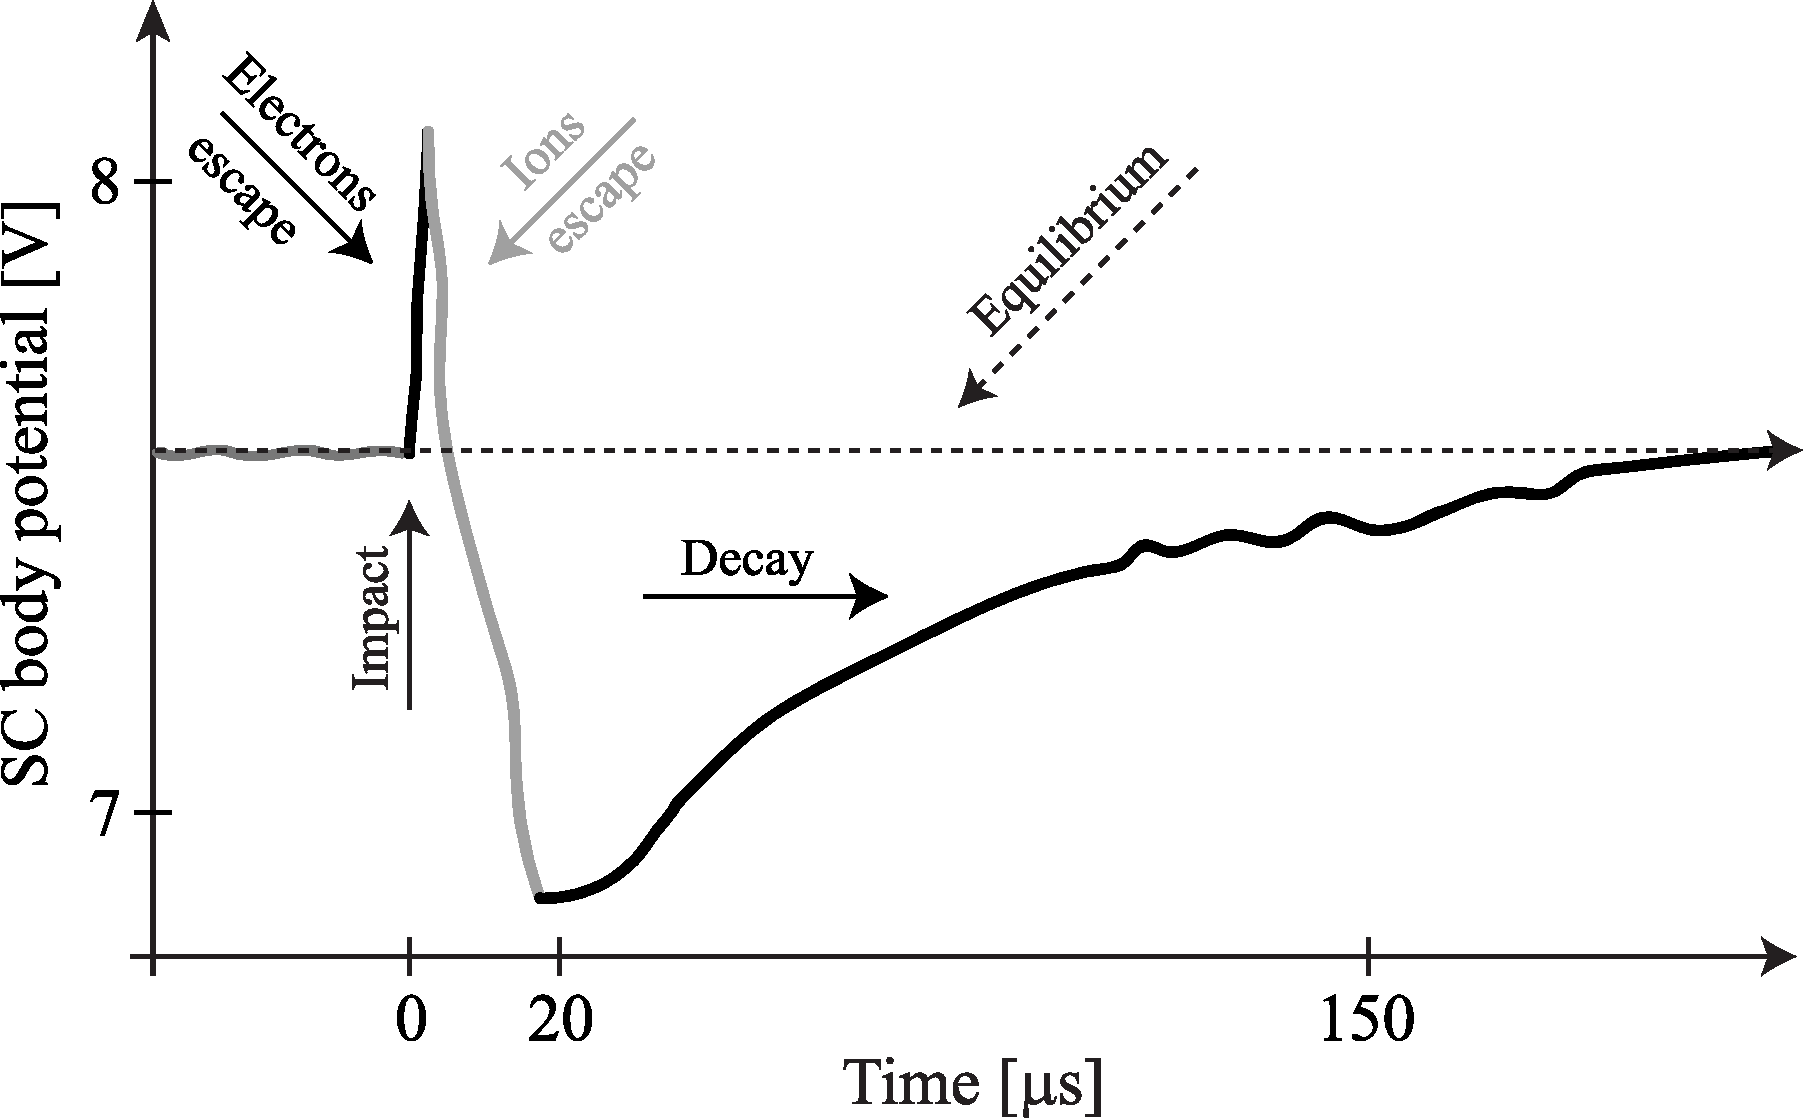
\includegraphics[width=8cm]{figures/impact_wf_gs.pdf}
 	\caption{A~simplified dust impact monopole electrical signature after an impact onto a~positively charged spacecraft body.}
 	\label{fig:impact_process}
\end{figure}

Therefore, there are several features to look for in the~time-domain measurements, such as the~quick rise of the~signal, and the~exponential decay of the~maximum. Visual identification is robust to the~extent to which experts' opinions on the~impact shape agree. Such identification is however very time consuming, and for a~big data set, it is clearly not feasible to use this method alone. 

This method is often regarded as the~standard (benchmark) for any other electrical antenna dust identification method since for spacecraft data, the~true information whether an impact happened, is not available. We also used this approximation in Paper~I. The expert visual classification, albeit imperfect, is by definition the~most reliable approximation of the~truth.

\subsubsection{Hard-coded identification}

The~features of dust impact signatures can be translated into algorithmic criteria, which are then efficiently applied to a~big data set. While these identification criteria work well for textbook examples of dust impacts, the~actual impacts in space may be quite different from the~canonical example, as they might contain a~lot of noise, saturated data, solitary waves, or a~superposition of a~dust impact and a~wave, and other non-standard signals \citep{vaverka2018comparison,ye2019understanding,malaspina2023dust}. One such algorithm is used for on-board identification of dust impacts on SolO \citep{maksimovic2020solar}, and in Paper~I, we found this algorithm to be $\SI{85}{\%}$ accurate and $\SI{75}{\%}$ precise. The~test was performed on a~sample containing $\SI{50}{\%}$ dust and $\SI{50}{\%}$ non-dust recordings, as assigned by the~tested algorithm. Classification performance improvement was the~main motivation for the~development of a~more reliable automatic identification procedure presented in Paper~I. 

\subsubsection{Machine learning}

Supervised machine learning has established itself as a~method of time-series classification, particularly in cases, when the~exact classification criteria are hard to formulate, but labelled data are abundant \citep{wickstrom2022mixing}. This makes it suitable for the~problem of dust identification. Methods are available, such as support vector machine ({SVM}), which evaluates a~set of pre-defined quantitative features on labelled data and creates a~decision algorithm based on them \citep{vapnik1997support}. Convolutional neural network ({CNN}) is a~type of a~neural network particularly useful for the~classification of grid-like objects, such as images or time-series \citep{gu2018recent}. Unlike SVMs, CNNs yield the~features vector by convolution operations, and therefore, they do not require a~pre-defined feature extracting routine. One common disadvantage of neural networks ({NN}s), including CNNs, is that their decision making might be difficult to explain, as NNs generally are black boxes, with their internal working hard to interpret. However, great progress in NN explainability was achieved, at least for a~limited class of CNNs, in the~recent past \citep{samek2021explaining}. If designed to be so, CNN can be explainable to the~extent that even features with non-linear effects are interpretable. This not only mitigates the~black box trust issue but provides more insight into the~problem. In Paper~I, both an SVM and an explainable CNN were successfully used to meaningfully improve the~performance of the~dust identification algorithm, compared to the~on-board hard-coded algorithm. The~best performing CNN model showed $\SI{96}{\%}$ accuracy and $\SI{94}{\%}$ precision on a~balance sample.

\section{Dust detection flux modelling}

With antenna detection of dust impacts, the~whole body of the~spacecraft acts as a~detection surface for collisions between dust grains and the~spacecraft. Assuming a~6D phase space probability density function $f(\vec{r},\vec{v})$ for the~dust cloud composed of grains of identical mass, where $\vec{r}$ is the~location and $\vec{v}$ is the~velocity of the~dust, and normalized to dust number density $n$ as
\begin{equation}
    n(\vec{r}) = \iiint_{\mathbb{R}^3} f(\vec{r},\vec{v}) \,dv_x\,dv_y\,dv_z,
\end{equation}
and a~spherical spacecraft with the~cross section of $S$, the~detection rate $\lambda$ is
\begin{equation}
    \lambda(\vec{r}) = S \iiint_{\mathbb{R}^3} |\vec{v}-\vec{v}_{sc}| f(\vec{r},\vec{v})  \,dv_x\,dv_y\,dv_z, \label{eq:phase_space_lambda}
\end{equation}
assuming the~spacecraft speed $\vec{v}_{sc}$. If the~spacecraft moves through a~dust cloud with a~sharp relative speed between the~spacecraft and the~dust $v_{imp}=|\vec{v}_{sc}-\vec{v}|$, which is provided by the~dust grains having the~same velocity $\vec{v}$:
\begin{equation}
    \iiint_{\mathbb{R}^3} f(\vec{r},\vec{v}) \,dx\,dy\,dz = \delta(\vec{v}),
\end{equation}
the detection rate simplifies to  
\begin{equation}
    \lambda = S n v_{imp},
\end{equation}
assuming that the~local number density of dust is $n$ and that all the~grains are detected, if collided with. In reality, the~dust cloud is not composed of grains of identical mass. Therefore, all the~collisions are never registered, and the~higher relative speed $v_{imp}$ implies a~higher charge produced on impact (Eq.~\ref{eq:charge_generation}), and in turn higher probability of detection, therefore the~rate is sometimes modelled as
\begin{equation}
    \lambda = S n v_{imp}^{1+\alpha \delta}, \label{eq:rate_semi_general}
\end{equation}
where $\alpha$ is the~parameter in charge generation (Eq.~\ref{eq:charge_generation}), and $\delta$ is the~mass distribution slope (Eq.~\ref{eq:mass_distribution}). 

Eq.~\ref{eq:rate_semi_general} can be simplified for different dust populations. For example, for bound dust, there is a~bond between the~dust speed $\vec{v}$ and the~heliocentric distance $r$ \citep{szalay2020near}. For $\beta$-meteoroids sufficiently far from the~Sun, $\vec{v}$ can be reasonably assumed radial and with a~speed $v$, which does not depend on $\vec{r}$ \citep{zaslavsky2021first}. For both bound dust and $\beta$-meteoroids, $n$ depends only depends on the~heliocentric distance $r$ (Eqs.~\ref{eq:dust_number_density} and \ref{eq:beta_number_density}). For interstellar dust, $n$ and $\vec{v}$ are sometimes assumed constant and homogeneous, which is often compatible with the~data \citep{babic2022situ}. In principle, the~cross section $S$ in Eq.~\ref{eq:rate_semi_general} is orientation dependent for non-spherical spacecraft. 
The~total model rate $\Lambda$ in a~multi-component model is a~superposition of the~detection rates $\lambda_i$ for each of the~modelled populations as
\begin{equation}
    \Lambda = \sum_{\forall i} \lambda_i, \label{eq:multiple_copmonent}
\end{equation}
where each individual $\lambda_i$ is reasonably approximated. 

In Paper~II, we decided to explain the~flux observed on SolO with a~two-component, semi-empirical model (as in Eq.~\ref{eq:multiple_copmonent}). This way, we were able to constrain some of the~parameters of the~$\beta$-meteoroids, such as their speed and acceleration. In Paper~IV, we built a~physics based model for bound dust detections on PSP, using the~phase space distribution approach (Eq.~\ref{eq:phase_space_lambda}) and we were able to constrain some of the~orbital parameters of the~near-solar dust. 

\subsection{Orbital parameters and the~data set}

Depending on the~orbit of a~spacecraft, the~observed dust flux is dependent on, and therefore holds the~information about different dust populations, while being unable to resolve other populations. We discussed the~defining properties of common dust populations in Ch.~\ref{ch:populations}. The~orbits of selected spacecraft are shown in Fig.~\ref{fig:sc_orbits}. In this section, we present different spacecraft, and we explain why their measurements complement each other.  

\begin{figure}[hb]
 	\centering
 	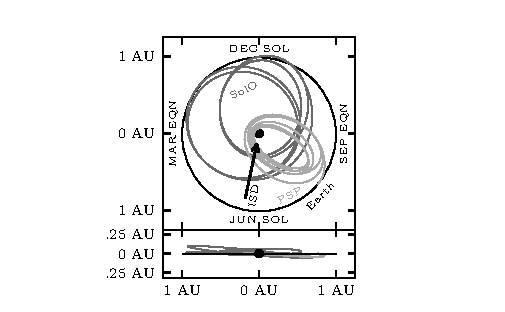
\includegraphics[width=13cm]{figures/solo_orbit.pdf}
 	\caption{The~orbit of SolO and PSP in heliocentric (HAE) coordinates between their respective launch date and the~summer of 2024, shown in $XY$ (top) and $XZ$ (bottom) planes. The~orbit of the~Earth is shown for reference, which is very similar to the~orbits of the~two STEREO spacecraft. The~direction of ISD flow is shown with an arrow.}
 	\label{fig:sc_orbits}
\end{figure}

\subsubsection{Solar Terrestrial Relations Observatory}

The~two STEREO spacecraft orbit the~Sun on a~nearly circular orbits close to $\SI{1}{AU}$. Their electrical antenna measurements allow for dust identification \citep{meyer2009dust}. Beyond the~intermittent and hard to explain nanodust \citep{meyer2009dust}, the~flux was found to be dominated by $\beta$-meteoroids \citep{zaslavsky2012interplanetary}. However, distinguishing $\beta$-meteoroids from bound dust is virtually impossible, since, owing to the~circular orbit, the~flux of both is expected to be constant throughout the~orbit and the~years. This is also an advantage for the~detection of interstellar dust (ISD), which is directional, and even though its flux is relatively low, compared to $\beta$-meteoroids, it causes most of the~observed variance \citep{zaslavsky2012interplanetary,malaspina2015revisiting,babic2022situ}, with the~flux maxima coinciding with the~anti-parallel velocity between STEREO and ISD, and minima coinciding with the~parallel configuration. Like STEREO, the~spacecraft located in Earth's L1 point also exhibit a~nearly-constant $\beta$-meteoroid and bound dust fluxes and are in a~good position to investigate ISD \citep{malaspina2014interplanetary,malaspina2016database}.

\subsubsection{Solar Orbiter}

SolO orbits the~Sun on an elliptical orbit between $\SI{0.3}{AU}$ and $\SI{1}{AU}$ (eccentricity $e \approx 0.52$ in 2024), which means that neither its exposure to bound dust, nor $\beta$-meteoroids is constant. This makes identification of ISD difficult, as it is no longer responsible for an important part of the~observed variance. However, the~$\beta$-meteoroids are clearly apparent, since the~spacecraft's radial speed alternates between negative (pre-perihelia) and positive (post-perihelia), which changes the~incidence between the~spacecraft and the~outgoing $\beta$-meteoroids. Asymmetry in the~flux between the~inbound and the~outbound leg allowed for some of the~$\beta$-meteoroid parameters to be constrained by \citet{zaslavsky2021first} and in Paper~II. The~$\beta$-meteoroids are dominant in the~SolO data to the~extent that it is not even clear from SolO data alone that bound dust is needed to explain the~observed flux.

\subsubsection{Parker Solar Probe}

The~orbit of PSP is even more eccentric ($e \approx 0.86$ in 2024), compared to SolO, but even more importantly, PSP gets as close as $\SI{0.052}{AU}$ from the~Sun. The~relative speed between PSP and the~dust components was evaluated by \citet{szalay2020near}, and all suggests that unlike for any other spacecraft, the~near-solar dust flux is dominated by bound dust impacts, especially in the~post-perihelia. While ISD is difficult to distinguish in SolO data, it is very unlikely to be confidently identified in PSP data, since the~variation of the~flux on PSP is even much higher, and the~alignment is even more unfortunate, with the~likely peak of ISD impacts being nearly aligned with the~perihelia (see Fig.~\ref{fig:sc_orbits}). The~bound dust component, crucial for the~flux modelling on PSP, was modelled and constrained in Paper~IV. In the~paper, we also discuss the~different material of the~heat shield, and how it likely causes the~heat shield to be less sensitive to the~impacts. The~great variability of the~ambient conditions poses additional challenges, as the~electric potential, and even conductivity of the~spacecraft changes throughout each orbit significantly, which we also investigated and discussed in Paper~IV.

\subsection{Compatibility of Solar Orbiter and Parker Solar Probe dust data}

In Paper~II, we presented a~Bayesian fit of a~semi empirical dust flux model to the~SolO data from between 6/2020 and 12/2021. As a~natural continuation of that effort, in this section we build on that model, and adjust the~procedure from Paper~II. We perform a~similar fit but done using the~aggregated SolO data from between 6/2020 and 6/2023 and PSP data from between 10/2018 and 7/2023. As we will see, a~good fit is possible, but it does not yield much new information about the~dust cloud.

Since the~goal of this section is to incorporate measurements from PSP, the~model needs to change with respect to the~model used in Paper~II, as there are physical differences between the~spacecraft. Having more data, however, we can afford to fit a~somewhat more complicated model, working with six unknowns (hyperparameters). The~changes with respect to Paper~II are:
\begin{itemize}
    \item a~two-component model assuming $\beta$-meteoroids and bound dust is used, as opposed to the~two-component model assuming $\beta$-meteoroids and a~constant background rate used in Paper~II,
    \item a~cuboid shape is assumed for both spacecraft with a~different cross section from the~front, from the~side, and from the~back, assuming a~motion in the~plane of ecliptic, 
    \item while in the~case of SolO, the~cross sections from the~front and from the~back are assumed equal, in the~case of PSP, the~front side is assumed to have a~smaller cross section, due to a~different material of the~heat shield, as discussed in Paper~IV.
\end{itemize}

\begin{table}[t]
\caption{The~cuboid-approximation cross section for SolO and PSP. Front side means the~sunward side, back is the~opposing side. $\alpha_{shield}$ is the~PSP heat shield miss rate parameter.}
\centering
\label{tab:cross_section}
\begin{tabular}{c|ccc}
\multicolumn{1}{p{1.2cm}}{  } \vline &  
\multicolumn{1}{p{3cm}}{ \centering $S_{front} \, [m^2]$ } & 
\multicolumn{1}{p{2cm}}{ \centering $S_{side} \, [m^2]$} & 
\multicolumn{1}{p{2cm}}{ \centering $S_{back} \, [m^2]$} \\
\hline
SolO & $10.34$ & $8.24$ & $10.34$   \\
PSP & $6.11 \cdot (1-\alpha_{shield})$ & $4.62$ & $6.11$  \\
\hline
\end{tabular}
\end{table}

We model the~detection count per day in the~case of SolO and per eight hours in the~case of PSP. This choice is not very consequential, if it is reasonable to assume the~detection rate constant within one detection interval, and if an appropriate procedure is used. The~SolO/RPW data is a~product of the~CNN procedure presented in Paper~I and the~PSP/FIELDS data is the~data product by \citet{malaspina2023dust}, which is the~same data product as used in Paper~IV. The~detection count is assumed to come from a~Poisson distribution (as in Eq.~\ref{eq:poisson_pmf}) and the~six-parameter model for the~rate, with the~free parameters $\lambda_a, \lambda_b, v_{b,r}, \epsilon_v, \epsilon_{b,r}, \alpha_{shield}$ is 
\begin{equation}
    \Lambda = E (\lambda_{bound} + \lambda_{\beta}),
\end{equation}
where $E$ is the~exposure time, and the~components $\lambda_{bound},\lambda_{\beta}$ are
\begin{equation}\begin{split}
    \lambda_{bound} &= \lambda_a  S(sc,\phi{a}) \left( \frac{|\vec{v}_{a} - \vec{v}_{sc}|}{v_{a,norm}}\right)^{\epsilon_v} \left( \frac{R}{\SI{1}{AU}} \right)^{-1.3} \\
    \lambda_{\beta} &= \lambda_b S(sc,\phi{b}) \left( \frac{|\vec{v}_{b} - \vec{v}_{sc}|}{v_{b,norm}}\right)^{\epsilon_v} \left( \frac{R}{\SI{1}{AU}} \right)^{\epsilon_{b,r}},
\end{split}\end{equation}
where $R$ is the~heliocentric distance, and $S(sc,\alpha)$ is the~effective cross section, dependent on the~spacecraft and the~incident angle $\phi$, which in turn depends on the~velocity of the~dust cloud $\vec{v}_a,\vec{v}_b$ and of the~spacecraft $\vec{v}_{sc}$. For compactness, the~subscripts $a$ and $b$ correspond to bound dust and $\beta$-meteoroids, respectively. The~bound dust velocity $\vec{v}_a$ is assumed to be purely azimuthal with the~speed
\begin{equation}
    |\vec{v}_a| = \left( \frac{R}{\SI{1}{AU}} \right)^\frac{1}{2} \cdot \SI{29.8}{kms^{-1}},
\end{equation}
while the~velocity of $\beta$ has two components
\begin{equation}\begin{split}
    \vec{v}_b &= \vec{e}_{rad} v_{b,rad} + \vec{e}_{azim} v_{b,azim} \\
    v_{b,rad} &= \left( \frac{R}{\SI{1}{AU}} \right)^{-2-\epsilon_{b,r}} \, v_{b,r} \\
    v_{b,azim} &= \frac{R}{\SI{1}{AU}} \cdot \SI{9}{kms^{-1}}.
\end{split}\end{equation}
Finally, the~speed normalization is done with respect to a~stationary (non-orbiting) object at $\SI{1}{AU}$, therefore
\begin{equation}\begin{split}
    v_{a,norm} & = \SI{29.8}{kms^{-1}} \\
    v_{b,norm} & = \left( v_{b,r}^2 + \left(\SI{9}{kms^{-1}}\right)^2 \right)^\frac{1}{2},
\end{split}\end{equation}
where the~speed of $\beta$-meteoroids at $\SI{1}{AU}$ of \SI{9}{kms^{-1}} is based on a~discussion in Paper~II. In this case, the~fit was performed by M-H MCMC sampling. The~assumed cross sections are based on the~projections of the~3D models \citep{psp_model,solo_model} of the~two spacecraft and are summarized in Tab.~\ref{tab:cross_section}.

\begin{figure}[ht]
 	\centering
 	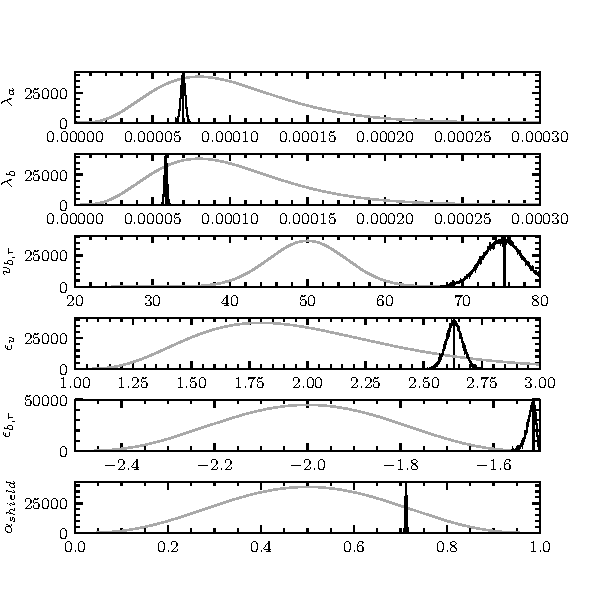
\includegraphics[width=9cm]{figures/both_shield.pdf}
 	\caption{The~marginals of the~prior (gray) and the~posterior (black) of the~fit. The~posterior is based on a~sample of $10^7$ points and the~MAP values are indicated with vertical lines. Neither prior nor the~posterior are normalized. The~summary of both is shown in Tab.~\ref{tab:prior_posterior}.}
 	\label{fig:fit_posteriors}
\end{figure}

\begin{table}[t]
\caption{The~summary of the~prior and the~posterior marginals, the~same as shown in Fig.~\ref{fig:fit_posteriors}.}
\centering
\label{tab:prior_posterior}
\begin{tabular}{c|cc|cc}
\multicolumn{1}{c}{  } \vline & \multicolumn{2}{c}{prior} \vline & \multicolumn{2}{c}{posterior} \\ 
& distribution & support & mean & st. dev. \\
\hline
$\lambda_a$ & $\Gamma(k=5,\theta=2\cdot10^{-5})$ & $\mathbb{R}^+$ &
$6.97 \cdot 10^{-5}$ & $1.4 \cdot 10^{-6}$  \\
$\lambda_b$ & $\Gamma(k=5,\theta=2\cdot10^{-5})$ & $\mathbb{R}^+$ & 
$5.85 \cdot 10^{-5}$ & $8.2 \cdot 10^{-7}$  \\
$v_{b,r}$ & $Norm(\mu=50,\sigma=5)$ & $\mathbb{R}$ & 
$75.3$ & $2.7$  \\
$\epsilon_v$ & $1+\Gamma(k=5,\theta=2\cdot10^{-1})$ & $(1,\infty)$ &
$1.63$ & $3.5 \cdot 10^{-2}$  \\
$\epsilon_{b,r}$ & $-1.5-B(\alpha=4,\beta=4)$ & $(-2.5,-1.5)$ &
$-1.52$ & $9.6 \cdot 10^{-3}$  \\
$\alpha_{shield}$ & $B(\alpha=4,\beta=4)$ & $(0,1)$ & 
$0.71$ & $1.4 \cdot 10^{-3}$  \\
\hline
\end{tabular}
\end{table}

The~main shortcomings of the~model are the~single dust speed assumed, the~cuboid approximation, and the~approximation of $\lambda_\beta \propto R^{\epsilon_{b,r}}$. The~dimension of the~model, six, is quite high. Therefore, we constrained the~support of the~hyperparameters wherever reasonable. This is done with the~transformations used for the~prior, indicated in Tab.~\ref{tab:prior_posterior}. This constraint is most apparent in the~value of $\epsilon_{b,r}$ being close to the~support boundary, which indicates a~deficient model, perhaps on the~assumption of a~single $\beta$-meteoroid speed at each heliocentric distance. However, we note that in Paper~II, the~posterior mean of the~corresponding parameter $\epsilon_r$ was found to be $-1.61$ with the~standard deviation of $0.16$, hence, compatible with the~present result, even as the~prior support spanned $\mathbb{R}$.

The~priors and posteriors are shown in Fig.~\ref{fig:fit_posteriors} and summarized in Tab.~\ref{tab:prior_posterior}. They are somewhat different from the~results of Paper~II, but this is to be expected, since the~data is different, as is the~model. Therefore, the~unknown parameters do not have the~exact same meaning as they had in Paper~II. The~conclusions drawn from the~fit in Paper~II would not be substantially different if they were to be drawn from this fit. Interestingly, the~PSP heat shield miss rate parameter $\alpha_{shield}$ implies that the~sensitivity of the~PSP's front side is by a~factor of nearly four lower than the~sensitivity of its other sides, and that of SolO. Two things are apparent from Fig.~\ref{fig:fit_rate}. First, the~model predicts that there is a~period present in each post perihelion of PSP, when bound dust dominates the~flux, consistently with the~predictions made by \citep{szalay2020near,szalay2021collisional}. This supports the~validity of the~analysis done in Paper~IV. This is not observed for SolO, for which $\beta$-meteoroids are always dominant. Second, the~model is deficient, as it fails to represent the~aphelia fluxes of later PSP orbits, where the~model flux is higher than observed. This might be an instrumental effect, if the~change of the~spacecraft's sensitivity introduces variance beyond what is a~part of the~model, but it might be a~sign that the~model does not sufficiently capture the~dynamics of the~dust cloud. We however see that both spacecraft do fit well in the~same framework of a~two-component, $\beta$ and bound dust model. 

\begin{figure}[hb]
 	\centering
 	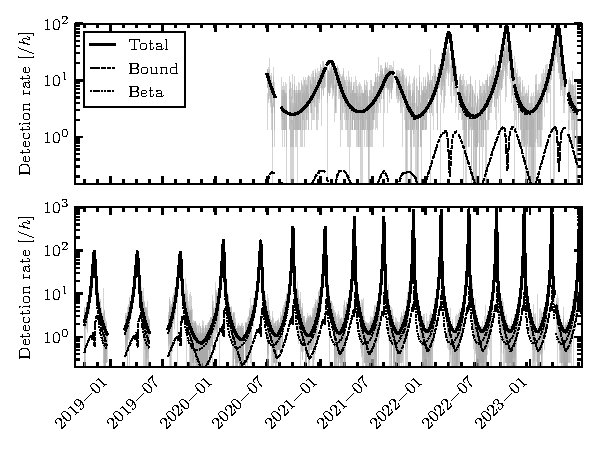
\includegraphics[width=12cm]{figures/both_shield_rate_log.pdf}
 	\caption{The~measured impact rate for SolO (top) and PSP (bottom), where the~error bars correspond, for visualization purposes, to $\SI{90}{\%}$ confidence intervals, assuming the~rate was identical to the~observed count per exposure time. The~lines correspond to the~MAP result of the~two-component fit.}
 	\label{fig:fit_rate}
\end{figure}







